\documentclass{standalone}

\usepackage{amssymb}
\usepackage{tikz}
%\usepackage{pst-all}              % pstricks, alle Pakete


\begin{document}
\usetikzlibrary {positioning}

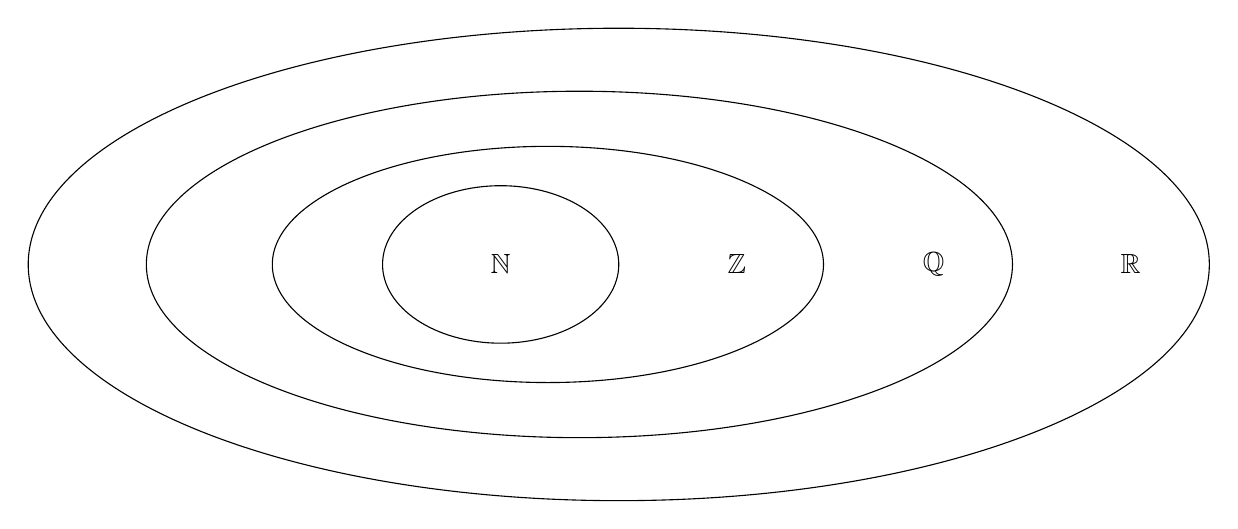
\begin{tikzpicture}
	\draw (0,0) ellipse [x radius=1.5, y radius = 1];
	\node at (0,0) {$\mathbb{N}$};
	
	\draw (0.6,0) ellipse [x radius=3.5, y radius = 1.5];
	\node at (3,0) {$\mathbb{Z}$};
	
	\draw (1,0) ellipse [x radius=5.5, y radius = 2.2];
	\node at (5.5,0) {$\mathbb{Q}$};

	\draw (1.5,0) ellipse [x radius=7.5, y radius = 3];
	\node at (8,0) {$\mathbb{R}$};

\end{tikzpicture}

\end{document}